\documentclass[a4paper]{article}
\usepackage[left=2cm,right=2cm,top=3cm,bottom=3cm]{geometry}
\usepackage[T1]{fontenc}
\usepackage{amsmath}
\usepackage{mathtools}
\usepackage{amssymb}
\usepackage{indentfirst}
\usepackage{graphicx}
\usepackage{algorithm}
\usepackage{algorithmic}
\graphicspath{ {./images/} }

\title{\textbf{Pracownia z Analizy Numerycznej}\\{\Large Sprawozdanie do zadania P1.7}}
\author{Mateusz Leonowicz}

\begin{document}
\maketitle

\section{Wstęp}
    Wiele problemów w matematyce, fizyce czy informatyce sprowadzić można do wyznaczenia miejsc
    zerowych danego równania algebraicznego. Często nie wystarczy nam prosta analiza funkcji, a
    jedyne co możemy zrobić, to obliczenie jej wartości w danej, skończonej liczbie punktów jej dziedziny.
    Dlatego temat ten stał się jednym z fundamentalnych zagadnień analizy numerycznej, dzięki czemu
    powstało wiele metod iteracyjnych, które oczywiście mają swoje zalety i wady.
    
    \vspace{5mm}

    Celem tego sprawozdania jest przedstawienie metod obliczania pierwiastków wielomianów w postaci
    \[ax^3 + bx^2 + cx + d = 0 \qquad a, b, c, d \in \mathbb{R}\]
    które pozwalają komputerom na uzyskanie wyników z kontrolowanym błędem. Przedstawię trzy metody numeryczne oraz 
    rozwiązania z użyciem wzorów Cardano. Opiszę ich działadnie i charakterystykę, a następnie umieszczę ich porównanie
    razem z podsumowaniem.

    Wszystkie testy przeprowadzane będą z użyciem języka do analizy numerycznej Julia.
    
\tableofcontents

\newpage
\section{Metoda Newtona}
    Niech $f(x)$ będzie funkcją, której miejsce zerowe chcemy wyznaczyć. Niech $\alpha$ będzie takim zerem, a $x$
    jego przybliżeniem. Z twierdzenia Taylora, wiemy, że przybliżenie funkcji $f$, możemy zapisać w postaci:
    \[
        0 = f(\alpha) = f(x + e) = f(x) + ef'(x) + \frac{f''(\xi)}{2!}e^2 \qquad \xi \in \text{interv}(x, \alpha) 
    \tag{1}\]

    Jeśli nasz wyraz $\frac{f''(\xi)}{2!}e^2$ będzie dostatecznie mały, to możemy go pominąć i rozwiązać równanie 
    względem $e$, co daje nam:
    \[
        e = \frac{-f(x)}{f'(x)}  
    \]

    Jeśli $x$ jest dostatecznie dobrym przybliżeniem $\alpha$, to $x - e$ będzie jeszcze lepszym przybliżeniem tego
    pierwiastka. Na tej różnicy opiera się metoda Newtona, która po wybraniu startowego przybliżenia $x_0$ zera $\alpha$
    polega na stosowaniu rekurencyjnego wzoru:
    \[
        x_{n+1} = x_n - \frac{f(x)}{f'(x)} \qquad n \geq 0
    \tag{2}\]

    Dobranie startowego punktu $x_0$ w tej metodzie jest bardzo istotne, gdyż metoda Newtona nie zawsze jest zbieżna.
    Jeśli dobierzemy odpowiednio punkt początkowy, to będziemy mieli zbieżność kwadratową (z wyjątkiem przypadków, gdy 
    istnieją wielokrotne zera funkcji. Wtedy otrzymamy zbieżność liniową).

    \vspace{5mm}

    Metoda Newtona opiera się na linearyzacji funkcji $f$, co pozwala nam na dobre przybliżanie wartości funkcji w małym
    otoczeniu punktu $x$. Możemy więc, rozumieć tę metodę, jako przybliżanie miejsc zerowych funkcji, za pomocą jej stycznych,
    co oczywiście niesie za sobą groźbę rozbieżności.

    \vspace{10mm}

    \begin{figure}[h]
        \centering
        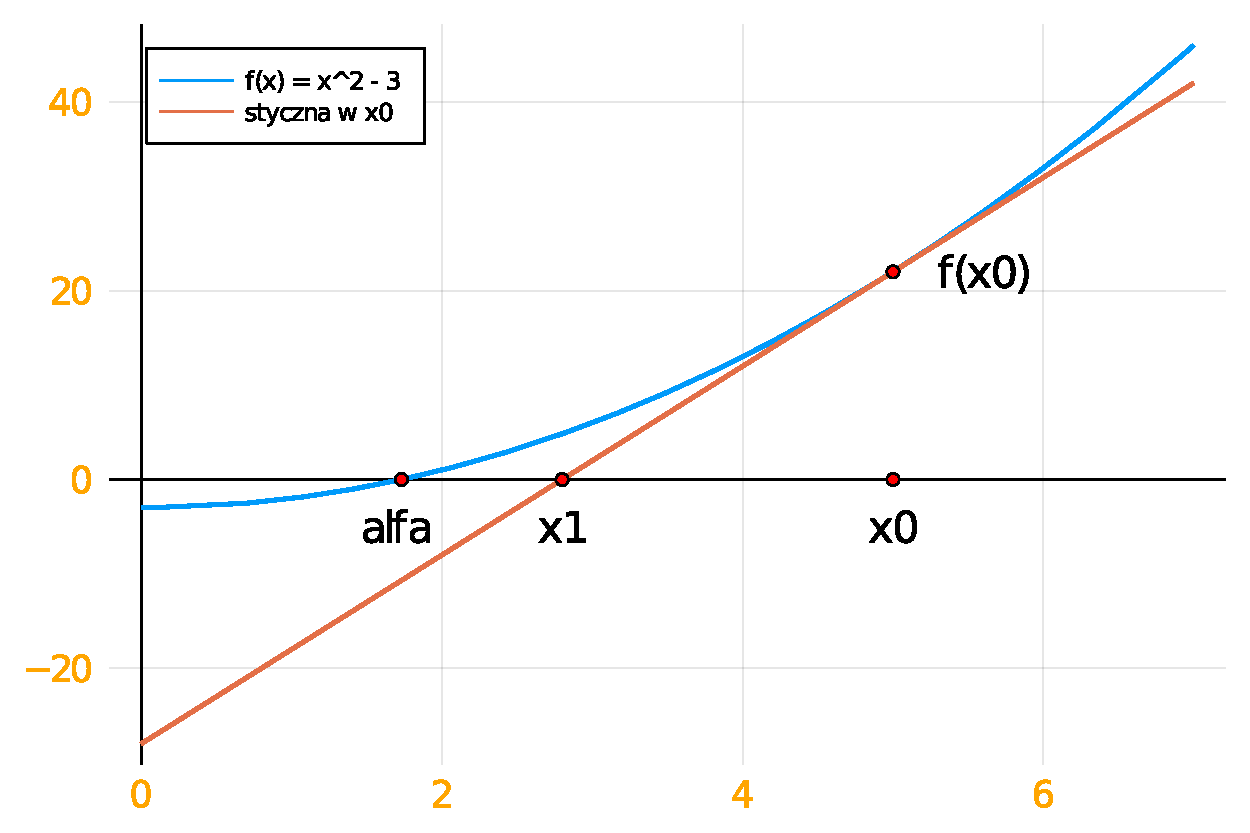
\includegraphics[width=12cm]{newtonPlot}
        \caption{Interpretacja geometryczna metody Netwona}
    \end{figure}

\newpage
\section{Metoda biskecji}
    Niech $f$ będzie funkcją ciągłą w przedziale $[a,b]$ i jeśli $f(a)f(b) < 0$, czyli funkcja zmienia znak na końcach przedziałów, to
    ta funkcja musi mieć zero w przedziale $(a,b)$ i jest to oczywiście konsekwencja twierdzenia Darboux. Możemy więc zmniejszyć nasz
    przedział o połowę wybierając punkt $c$, taki że $f(c)f(a) < 0$ lub $f(c)f(b) < 0$. Uzyskaliśmy nowy przedział, w którym wiemy, że
    znajduje się nasze miejsce zerowe. Na tym rozumowaniu opiera się metoda biskecji, którą wyrazić można następującym algorytmem:

    \begin{algorithm}
    \caption{Szukanie pierwiastka funkcji $f$}
    \begin{algorithmic}
    \REQUIRE $\epsilon\ a_0\ b_0\ M \quad \text{takie, że} \quad f(a_0)f(b_0) < 0$
        \STATE $n \leftarrow 1$
        \STATE $left \leftarrow a_0$
        \STATE $right \leftarrow b_0$
        \WHILE{$n < M$}
        \STATE $c = \frac{left + right}{2}$
        \IF{$f(c) = 0 \vee \lvert left - right \lvert < \epsilon$}
        \STATE $\text{pierwiastkiem jest}\ c$
        \ELSE
        \STATE $n \leftarrow n + 1$
        \ENDIF
        \IF{$f(left)f(c) < 0$}
        \STATE $left \leftarrow c$
        \ELSE
        \STATE $right \leftarrow c$
        \ENDIF
        \ENDWHILE
        \end{algorithmic}
    \end{algorithm}

    Algorytm uwzględnia trzy kryteria zakończenia obliczeń, ponieważ inaczej istniałoby
    ryzyko zapętlenia. Pierwszym jest oczywiście znalezienie takiego punkt $c$, że $f(c) = 0$. Drugim z nich jest 
    skończona liczba iteracji, wyrażona zmienną $M$. Oprócz tego, obliczenia są przerywane, 
    jeżeli błąd jest dostatecznie mały, tj. mniejszy od $\epsilon$. Łatwo znaleźć przykłady funkcji, w których,
    brak któregoś z kryterów mógłby prowadzić do bardzo błędnych wyników. Dodatkowo metoda ta, daje zbieżność liniową,
    więc stanowi ona raczej ciekawostkę, aniżeli wartościową metodę numeryczną szukania pierwiastków.

    \begin{figure}[h]
        \centering
        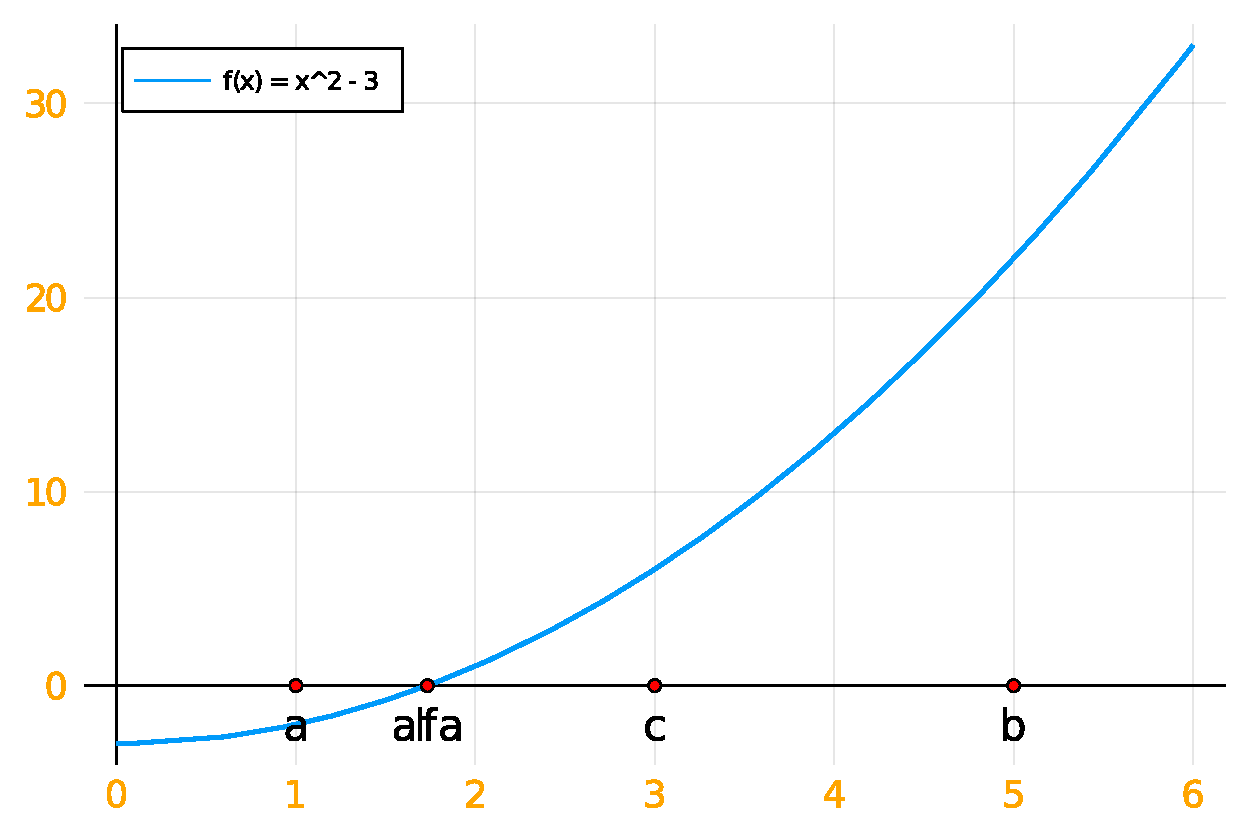
\includegraphics[width=12cm]{bisectionPlot}
        \caption{Interpretacja geometryczna metody bisekcji}
    \end{figure}

\newpage

\end{document}
